%%%%%%%%%%%%%%%%%%%%%%%%%%%%%%%%%%%%%%%%%
% Simple Sectioned Essay Template
% LaTeX Template
%
% This template has been downloaded from:
% http://www.latextemplates.com
%
% Note:
% The \lipsum[#] commands throughout this template generate dummy text
% to fill the template out. These commands should all be removed when 
% writing essay content.
%
%%%%%%%%%%%%%%%%%%%%%%%%%%%%%%%%%%%%%%%%%

%----------------------------------------------------------------------------------------
%	PACKAGES AND OTHER DOCUMENT CONFIGURATIONS
%----------------------------------------------------------------------------------------

\documentclass[12pt]{article} % Default font size is 12pt, it can be changed here

\usepackage[margin=1in]{geometry} % Required to change the page size to A4
\geometry{a4paper} % Set the page size to be A4 as opposed to the default US Letter

\usepackage{graphicx} % Required for including pictures

\usepackage{float} % Allows putting an [H] in \begin{figure} to specify the exact location of the figure
\usepackage{wrapfig} % Allows in-line images such as the example fish picture

\usepackage{lipsum} % Used for inserting dummy 'Lorem ipsum' text into the template

\usepackage{hyperref}
%\usepackage{apacite}
\usepackage{tikz}

\linespread{2} % Line spacing

%\setlength\parindent{0pt} % Uncomment to remove all indentation from paragraphs

\usepackage{soul} %for \hl to highlight
%\usepackage[final,inline,nomargin]{fixme}
\usepackage[draft,inline,nomargin]{fixme}
\newcommand{\hlfixme}[1]{\fxfatal{\hl{#1}}}
\newcommand{\hlfxnote}[1]{\fxnote{\hl{#1}}}

\graphicspath{{Pictures/}} % Specifies the directory where pictures are stored

\bibliographystyle{SIGCHI-Reference-Format}

\begin{document}

%----------------------------------------------------------------------------------------
%	TITLE PAGE
%----------------------------------------------------------------------------------------

\begin{titlepage}

\newcommand{\HRule}{\rule{\linewidth}{0.5mm}} % Defines a new command for the horizontal lines, change thickness here

\center % Center everything on the page

\textsc{\LARGE New York University}\\[1.5cm] % Name of your university/college
\textsc{\Large Big Data: Critical Perspectives}\\[0.5cm] % Major heading such as course name
\textsc{\large Term Paper}\\[0.5cm] % Minor heading such as course title

\HRule \\[0.4cm]
{ \huge \bfseries Examining Predictive Policing, Traditional Policing and Due Process Through a Lens of Probability}\\[0.4cm] % Title of your document
\HRule \\[1.5cm]

\begin{minipage}{0.4\textwidth}
\begin{flushleft} \large
\emph{Author:}\\
Kevin \textsc{Gallagher} % Your name
\end{flushleft}
\end{minipage}
~
\begin{minipage}{0.4\textwidth}
\begin{flushright} \large
\emph{Professor:} \\
Helen \textsc{Nissenbaum} % Supervisor's Name
\end{flushright}
\end{minipage}\\[4cm]

{\large \today}\\[3cm] % Date, change the \today to a set date if you want to be precise

%\includegraphics{Logo}\\[1cm] % Include a department/university logo - this will require the graphicx package

\vfill % Fill the rest of the page with whitespace

\end{titlepage}

%----------------------------------------------------------------------------------------
%	TABLE OF CONTENTS
%----------------------------------------------------------------------------------------
\clearpage\thispagestyle{empty}\addtocounter{page}{-1}
\tableofcontents % Include a table of contents
\newpage % Begins the essay on a new page instead of on the same page as the table of contents 

%----------------------------------------------------------------------------------------
%	INTRODUCTION
%----------------------------------------------------------------------------------------

\begin{abstract}
Big data, or the use of large quantities of data to make inferences and predictions of various interests, is slowly finding its way into many different aspects of daily life. Big data is used to recommend things such as television shows, music, to serve us promotions and advertisements, and even to score us on our ability to repay loans. 

Perhaps one of the most interesting applications of big data is predictive policing, or using large quantities of data to aid in policing tasks such as locating likely areas of crime, and determining who is likely to commit a serious crime in the near future. Though this application can help police more effectively perform their duty, it has also prompted many questions as to its affect on due process.

In the literature surrounding predictive policing, many papers claim that big data is a game changer for policing department, with some arguing that it will help society become a safer place while others argue that it opens many new avenues for the violation of civil rights. Despite these claims, to this author's knowledge no comparison between predictive policing and traditional law enforcement has yet been performed. This paper attempts to fill this looming gap in the research.

This paper compares and contrasts predictive policing and traditional law enforcement methods through a lens of probability, paying specific attention to potential impacts on due process and legal standards such as probable cause and reasonable suspicion. As part of this, this paper offers a novel probability based definition of reasonable suspicion and probable cause. In addition, differences and similarities of traditional policing methods and predictive policing are presented, including a novel observation about differences caused by machine learning's static feature space. Lastly, recommendations on future research are presented.
\end{abstract}
\newpage
\section{Introduction}\label{sec:introduction} % Major section

One Friday morning in July of 2011, two women were arrested in Santa Cruz, California after being caught peering into cars parked in a local parking garage. In addition to the suspicious nature of their activities, one of the women arrested had outstanding warrants, and the other was in possession of drugs. Though arrests of this nature are rarely reported on the news, this particular arrest was an exception due to its peculiar circumstances. These arrests were made after officers were dispatched because a computer algorithm predicted the area as likely to be affected by crime. \cite{nyt} 
This technology, called Predictive Policing, is defined as the application of analytical techniques, particularly quantitative techniques, to identify promising targets for police intervention and prevent or solve crime. \cite{perryetal} As such, predictive policing can be seen as a branch of ``Big Data'' or ``Data Science,'' the collection and analysis of large quantities of data to form predictive tools.

Since its inception, predictive policing has been a controversial topic. To many individuals, the idea of predicting crimes before they occur bring visions of a dystopia akin to that demonstrated by the film \textit{Minority Report}. To others, predictive policing is a new era of policing techniques, bringing what was becoming an outdated profession into the modern world. Despite the differences in their arguments, one who reads the predictive policing literature is bound to find one assertion on both sides, ``predictive policing will change everything.'' Despite these claims, to this author's knowledge no comparison between predictive policing and traditional policing method yet exists. In order to address this gap in the research, the purpose of this paper is to compare and contrast predictive policing and traditional policing techniques, paying specific attention to how they affect civil rights and due process. 

To achieve this goal, the effects of predictive policing will be viewed through a multidisciplinary lens. This paper discusses the definition of due process and its role in liberal democracies, the role of cognitive psychology and models of human thought in traditional policing, and the inner workings of machine learning and its role in predictive policing. In order to tie all of these different disciplines together, this paper discusses them all through the lens of probability and likelihood.

The remainder of this paper will be organized as follows, Section \ref{subsec:predictivepolicing} will define predictive policing. Section \ref{subsec:dueprocess} will define due process and discuss its role in liberal democracies, as well as offer a novel definition of the reasonable suspicion and probable cause standards through the lens of probability. Though the role of probability in due process has been observed before \cite{ferguson2012predictive}, to this author's knowledge it has never been formally defined as such. Section \ref{subsec:cognitive} will introduce elements of cognitive psychology. Section \ref{subsec:machinelearning} will discuss machine learning and probability and their roles in predictive policing. Section \ref{sec:oldvnew} will discuss the differences between predictive policing and traditional policing, focusing on how they affect civil rights and due process. Finally, Section \ref{sec:conclusion} concludes.

%------------------------------------------------
\subsection{Predictive Policing: Definition and Taxonomy} \label{subsec:predictivepolicing}% Sub-section

As mentioned in Section \ref{sec:introduction}, predictive policing is defined by Perry et al. to be the application of analytical techniques, particularly quantitative techniques, to identify promising targets for police intervention and prevent or solve crime. In the report \textit{Predictive Policing: The role of crime forecasting in law enforcement operations}, Perry et al. present a taxonomy of predictive policing methods. This taxonomy breaks predictive policing into four categories: \cite{perryetal}

\begin{enumerate}
\item Methods for predicting future crimes
\item Methods for predicting future offenders
\item Methods for predicting perpetrator's identities
\item Methods for predicting victims of crimes
\end{enumerate}

Category one, methods for predicting future crimes, focuses on predicting the times and places in which crimes are anticipated to occur. Category two, methods for predicting future offenders, focuses on predicting individuals and groups that are ``at risk of offending in the future.'' Category three, methods for predicting perpetrator's identities, focuses on identifying individuals who have committed past crimes. Lastly category four, methods for predicting victims of crimes, focuses on predicting individuals and groups that are ``likely to become victims of crime.''

\subsection{Due Process} \label{subsec:dueprocess}
%\hlfixme{Introduce the ideas of due process here, and why they are important. Inclue defition from OED and do a quick lit review. Maybe ask Jessica.}
Due Process is defined by the Oxford English Dictionary (US Edition) to be ``[f]air treatment through the normal judicial system, especially as a citizen’s entitlement.'' In modern liberal democracies (such as the United States), due process serves an important role; Due process protects citizens from unfair treatment under the law. 

Liberal democracies have at the core of their philosophies the idea that every individual has equal protection of human rights, civil rights, civil liberties, and other political freedoms. Due process of law is therefore necessary to protect the core tenants of this philosophy, and to protect the rights of citizens from governments that seek to violate these rights. It ensures that the weak, poor and powerless have the same legal protections as the strong, wealthy and powerful, creating equal treatment under the law.

In the United States, due process of law is separated into two groups, procedural due process and substantive due process. Procedural due process focuses on rights that apply to government proceedings that may result in the denial of an individual's right to life, liberty or property \cite{wex_procedural}. As part of procedural due process, it is well accepted that the following rights apply: \cite{friendly}

\begin{enumerate}
\item An unbiased tribunal.
\item Notice of the proposed action and the grounds asserted for it.
\item Opportunity to present reasons why the proposed action should not be taken.
\item The right to present evidence, including the right to call witnesses.
\item The right to know opposing evidence.
\item The right to cross-examine adverse witnesses.
\item A decision based exclusively on the evidence presented.
\item Opportunity to be represented by counsel.
\item Requirement that the tribunal prepare a record of the evidence presented.
\item Requirement that the tribunal prepare written findings of fact and reasons for its decision.
\end{enumerate}

Substantive due process is ``[a] doctrine holding that the 5th and 14th Amendments require all governmental intrusions into fundamental rights and liberties be fair and reasonable and in furtherance of a legitimate governmental interest.'' \cite{wex_substantive} One part of substantive due process is the application of the Bill of Rights, which contains as part of it the Fourth Amendment, or the protection against unreasonable searches and seizures by the government.

In modern policing, two legal standards keep the actions of law enforcement agencies in check, reasonable suspicion and probable cause. Reasonable suspicion is the standard that must be met in order for law enforcement officials to justify brief stops and detentions, but not full searches. \cite{wex_suspicion} Reasonable suspicion must be based on ``specific and articulable facts... taken together with rational inferences from those facts,'' which must be associated with a particular individual. \cite{terry} In order to receive a warrant for a search or to make an arrest, a law enforcement agent must meet the standard of probable cause. Probable cause requires a ``reasonable basis for believing that a crime may have been committed (for an arrest) or when evidence of the crime is present in the place to be searched (for a search).'' \cite{wex_cause} These standards keep the police from arbitrarily targeting individuals for investigation of crimes, instead requiring reasons for the infringement on their rights.

\begin{figure}
\begin{center}
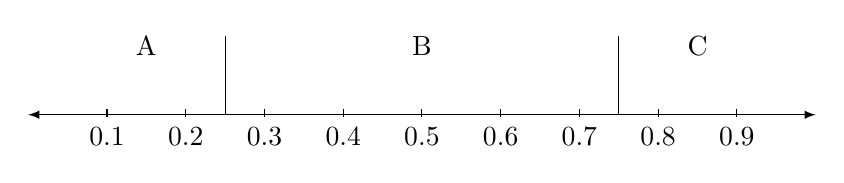
\begin{tikzpicture}
% a straight line segment
\draw[latex-latex] (0,0) -- (10,0);
% the ticks and their labels
\foreach \x  in {0.1,0.2,0.3,0.4,0.5,0.6,0.7,0.8,0.9}
  \draw[xshift=\x*10 cm] (0pt,2pt) -- (0pt,-1pt) node[below,fill=white] {\the\numexpr\x};
% the thicker segment
%\draw[ultra thick] (2.06,0) -- (8.94,0);
% the labels
%\node[fill=white,draw=black,circle,inner sep=2pt,label=above:{$p_1=.25$}] at (2.5,0) {};
%\node[fill=white,draw=black,circle,inner sep=2pt,label=above:{$p_2=.75$}] at (7.5,0) {};
%\node[fill=black,draw=black,circle,inner sep=2pt, label=below:{0} at (0,0) {};
%\node[fill=black,draw=black,circle,inner sep=2pt, label=below:{1} at (10,0) {};
%\node at (5.5,-0.8) {$\mu$};
\draw (2.5,0) -- (2.5,1);
\draw (7.5,0) -- (7.5,1);
\node [label=above:{A}] at (1.5,0.5) {};
\node [label=above:{B}] at (5,0.5) {};
\node [label=above:{C}] at (8.5,0.5) {};
\end{tikzpicture}
\caption{The number line separated into three sections by $p_1$ and $p_2$.}
\label{fig:numberline}
\end{center}
\end{figure}

To frame this into the discussion of probabilities, one can think of redefining reasonable suspicion and probable cause as probability threshold values $p_1$ and $p_2$ respectively, where $0 < p_1 < p_2 < 1$, where the values of $p_1$ and $p_2$ are defined by societal norms, legislation and case law. (Picking these values is not trivial, though the abstraction is still useful; picking the values of $p_1$ or $p_2$ will not be discussed further in this paper.) These values divide a number line on the interval [0,1] into three parts, as shown (with example values of $p_1$ and $p_2$) in Figure \ref{fig:numberline}. If the perceived probability $P$ (this term will be defined contextually in both Sections \ref{subsec:cognitive} and \ref{subsec:machinelearning}) is greater than $p_1$, but less than $p_2$, (i.e. $p_2 \geq P > p_1$), only the standard of reasonable suspicion is met. This can be seen as section B of the number line. If the perceived probability is above $p_2$ (i.e. $P > p_2$), the standards of probable cause and reasonable suspicion are met. This can be seen as section C of the number line. This reflects the fact that reasonable suspicion is a lesser standard than probable cause. If the perceived probability is less than $p_1$ (i.e. $P \leq p_1$), neither probable cause nor reasonable suspicion are met. This corresponds to section A of the number line. Though this numerical definition of these two standards may seem overly complex, they are necessary to tie together the areas of law, psychology and computer science discussed in this paper.

\subsection{Cognitive Psychology} \label{subsec:cognitive}
In order to understand judgements made by police before the creation of predictive policing, one must understand how to mind deals with decisions of a statistical nature. These ideas are detailed greatly by the work of Kahneman and Tversky, two psychologists who created and studied a useful model of human statistical thinking. This section briefly outlines the work done by Kahneman and Tversky in this field and is based entirely on Khaneman's book \textit{Thinking Fast and Slow}.\cite{kahneman}

In \textit{Thinking Fast and Slow}, Kahenman describes his work with Tversky in different areas of psychology. The central thesis of the book, and of Kahenman and Tversky's work itself, is the idea of a human's thought process being separated into two modes of thought, called ``system one and system two'' both in the academic literature and in the book itself. In the book, Kahneman explains that system one is fast and effortless. It acts as a statistician, counting occurrences and making quick predictions and reactions based on input stimuli. As such, it is trained over many years of input data and outcomes, calculating correlations and storing them for later use. System one is also responsible for expert reactions to domain specific problems. System two is the antithesis of system one. It is slow, effortful and logical, and it analyzes new problems and stimuli that system one was incapable of handling, or was proven to have handled incorrectly. Due to the effortful nature of system two, most decisions, predictions, judgements and reactions are made by system one, the quick and intuitive mode of thinking. In order to avoid activating the slow and effortful system two, there exist a list of heuristics that allow individuals to reach decisions using only system one, including framing, availability, loss aversion, and others.

Since system one is responsible for quick expert decisions, it is reasonable to believe that when a law enforcement agent attempts to assess whether a standard of probable cause or reasonable suspicion are met, they use the quick and intuitive ``statistician'' that is system one. To place this in context of the frame of probability, this can be viewed as a law enforcement agent estimates the perceived probability $P = f(x_1,...,x_n)$ (where each $x_i$ is a feature of the situation or context), that is the probability that an observed individual has committed or is going to commit a crime. This probability is estimated based on expert training (police training) and previous similar experiences. Then, the law enforcement agent estimates the values of $p_1$ and $p_2$ based on his or her understanding of the legislation and case law. Lastly, he or she compares the perceived probability $P$ with the thresholds $p_1$ and $p_2$ as described in Section \ref{subsec:dueprocess}.

%------------------------------------------------

\subsection{Machine Learning} \label{subsec:machinelearning}% Sub-section
In the age of big data, machine learning has taken on a large role in people's lives, though individuals are hardly aware of it. Machine learning allows companies and other groups to make predictions about what interests one is likely to have, what products one is likely to buy, and whether or not one is likely to repay his or her loans. In order to achieve this, the process of machine learning is broken down into four phases, feature creation, training, testing and prediction. The remainder of this section will describe the various phases of machine learning, drawing from the author's own knowledge and the textbook ``Introduction to Machine Learning'' by Ethem Alpaydin. \cite{introduction}

In the feature collection phase, historical data is obtained and formatted in a way that is useful for the machine learning algorithms. This is done by extracting information from a collected database that experts believe would be useful in training the machine learning algorithm for the purpose they are interested in (this will be discussed more in the following paragraphs). More precisely, given a database $D$, an algorithm or series of algorithms $f(D)$ is applied to the database and outputs a series of $N$ (where $N = size(D)$) vectors $x^{(j)} = {x_1, x_2, ..., x_m}$ where each $x_i$ s.t. $0 < i \leq m$ is said to be a feature, or attribute, of the data and $x^{(j)}$ s.t. $0 < j \leq N$ is said to be an instance of the data. 

After all entries in $D$ are converted to an instance of the data, the processes of feature selection and feature extraction are typically performed to reduce the number of features per instance. In feature selection, statistics about the features are calculated and the ones seen as less useful are discarded. In feature extraction, a combination of features is used to create a lower-dimensional representation. One example of this is Principle Component Analysis, which projects a combination of features onto a lower dimensional line. This allows for significantly less features with only slightly less performance accuracy. After these processes are performed, the output is an $N \times d$ matrix (where $d$ is the new number of features), which is called the training set. Given that there are $d$ features per entry (where $d \leq m$) in the training set, it is said that the feature space is $d$-dimensional. The next phases of the machine learning process depend on whether the goal of the algorithm is regression or classification. As such, the two will be discussed separately.

\subsubsection{Classification}
In machine learning classification, a business, government or other organization attempts to use historical data to place individuals into one of many categories. For example, an advertising company may want to place individuals into categories such as ``single male,'' or ``soccer mom,'' as the two groups are likely to consume very different products. To achieve this, the algorithm attempts to ``learn'' patterns in the training set and applies those learned patterns to data seen for the first time, picking the class that a particular set of feature values is most likely to be in. In supervised classification algorithms, this is done by labelling each vector $x^{(j)}$ with a ``correct'' output label, which is usually chosen by a domain expert or some sort of heuristic method. In this method, the accuracy of a machine learning classifier is determined based on how often it predicted this ``correct'' label. In unsupervised classification, feature vectors are grouped together based on some metric of similarity, for example the Euclidean distance when plotted. The advantage of this is that pre-labelled data is not necessary, but the downside is that accuracy can be hard to determine. There are many different algorithms for both supervised and unsupervised classification, some relying on separating data points with a line and others relying on discovering ``rules'' within the data to separate it into different classes. In every instance, however, the classifier is essentially outputting the same assertion, ``based on the data given, this set of data is more likely to belong to this class than any other.''

\subsubsection{Regression}
Unlike classification, where the only goal is to output a specific class, the goal of regression is to take in a set of features and output a number, which can be viewed as a score or an amount. One example of this is a credit score, which takes in information about one's debts, payments and other information and outputs a three digit score that is meant to convey how likely one is to repay his or her debts. Often, this is done by fitting a line or some other curve to the training data, and using the equation of that line for further predictions. Therefore, when a new set of data is seen it is simply plugged into the equation of the line or curve, thus getting a single number as an output. Accuracy is then determined by how far away the predicted value is from the ``real'' value using a standard error metric such as the sum squared error. There are many different methods of learning these lines or curves, and they are out of the scope of this paper. It is simple to see, however, that a regression algorithm can simply be turned into a classification algorithm by simply creating threshold values. For example, if a lender wanted to determine who to give a mortgage to, he or she could decide that the mortgage company will lend to anybody with a credit score of 700 and over, while denying anyone below that threshold. Therefore, the algorithm outputs only a score, and the classification decision is left to the humans interpreting it. 

\subsubsection{Machine Learning in Predictive Policing}
In predictive policing, machine learning is used to predict the likelihood of crime in a given neighborhood, the risk of an individual breaking his or her parole conditions, or other law enforcement related tasks. Specifically, historical data such as previous crimes in an area, previous crimes committed by an individual, modus operandi, etc is collected and then the feature creation stage is performed. Afterwards, these features are fed into classification or regression algorithms (depending on what is trying to be predicted). Lastly, the police analyze the output and determine if further action is required. In terms of the discussions of probability, reasonable suspicion and probable cause that appeared previously in this paper, one can view classification and regression as two methods of discovering a point on the due process number line. For a given situation, a classification algorithm could predict which section of the number line a situation falls into; either a situation falls into classes A, B or C as shown on the number line in Figure \ref{fig:numberline}. Alternatively, regression can be used to predict the perceived probability $P$ on the number line in Figure \ref{fig:numberline}, and then this point can be compared to the perceived thresholds and classified as potentially meeting one of the two standards. In practice today, however, predictive policing is not used solely to determine reasonable suspicion or probable cause. Instead, these things are used to redistribute police and visit persons predicted to be likely to commit crime. The following section will discuss the ways in which this is similar to previous methods of policing, and the ways in which this changes the policing field.
%----------------------------------------------------------------------------------------
%	MAJOR SECTION 1
%----------------------------------------------------------------------------------------

\section{The Novelty of Predictive Policing}\label{sec:oldvnew} % Major section
Big data technology, though promising and wondrous at first glance, has been the topic of many debates. This section will introduce some of the issues surrounding big data, and will then specifically discuss how these apply to the realm of policing. Afterwards, this section will explore the similarities and differences between predictive policing and traditional policing.

\subsection{Debates of Big Data}
Ever since the introduction of the concept of big data, there have been debates about its effectiveness and impact on social values. In general, many of the debates tend to focus around the areas of objectivity, transparency, discrimination, inaccuracies, and infringements on individual privacy (as the tracking created by dig data techniques can be even more intrusive than the aggregation of GPS data mentioned in US v Jones \cite{2012us}).

Many proponents of big data claim that one of its major strengths is its objectivity. This objectivity, as many claim, stems from the fact that mathematics and statistics are objective ways of measuring phenomena, and that building a classifier to uncover the correlations in this ``raw data'' is therefore objective as well. Some people, such as Chris Anderson, even goes as far as to claim that data science is the new scientific method, being even more objective than the previous models generated by the traditional scientific method. \cite{anderson_2008} Similarly believing in the objectivity of big data, Perry et. al liken the predictions made by predictive policing algorithms to forecasts, claiming that the word forecasting more accurately conveys the scientific objectivity that goes into the process. \cite{perryetal} On the other hand, there are many people, such as Moritz Hardt, who claim that big data is unfair, and ignores or even harms minority cases that are traditionally underprivileged. \cite{hardt} Another of these individuals is Lisa Gitelman, who claims that the idea of objectivity in ``raw data'' simply isn't factual, but rather that data is created and not measured. \cite{gitelman2013raw}

In the opinion of this author, it is true that there is a certain small amount of objectivity in machine learning, though it is limited. This objectivity is simply based on the fact that the machine learning algorithm will make its prediction based on the data it is provided and nothing else. This, however, is not sufficient to truly call machine learning or big data ``objective.'' Predictions are made based on historical data, which frequently reflects social biases. Features are selected based on input from experts, which, while more informed than lay people, are not immune from bias themselves. These introduced biases inevitably make their way into the predictions made by the algorithm, which may effect civil rights and due process in many ways. One example would be predicting minority areas as crime perpetrators, since individuals belonging to a minority group are incarcerated more frequently than others. \cite{naacp} One way this bias can be introduced is through numerical scoring methods such as the LSI-R. In the previously cited report by Perry et. al, the LSI-R, a scoring method used for determining conditions of one's parole, among other things, is presented as a possible feature for predictive policing algorithms. Though this may be viewed at a good thing at first glance, further investigation shows that this is an area where bias may be introduced. These LSI-R scores are created by humans evaluating other individuals, and often the bias introduced by this can even become procedure. For example, in the South Dekota Department of Human Service's LSI-R training slides, one of the included predictors of future crime is ``belonging to some minority groups.'' \cite{dekota} At the end of the processess this bias is obscured and forgotten about, since it is a lot easier for one to think of numbers entering a machine learning algorithm as an objective measurement, and disregarding where a feature originated.

In addition to the debate of objectivity, many discussions of big data also focus on the opaqueness inherent in big data.\cite{pasquale2015black} The following quote, taken from the same introductory machine learning book cited in Section \ref{subsec:machinelearning}, describes a motivation for finding a machine learning solution to the problem of spam detection. \cite{introduction}
\begin{quote}
``For some tasks, however, we do not have an algorithm—for example,
to tell spam emails from legitimate emails.  We know what the input is:
an email document that in the simplest case is a file of characters.  We
know what the output should be: a yes/no output indicating whether the
message is spam or not.  We do not know how to transform the input
to the output... 
What we lack in  knowledge,  we make up for in  data.   We can  easily
compile thousands of example messages some of which we know to be
spam and what we want is to ``learn'' what constitutes spam from them.''
\end{quote} 

Essentially, big data and machine learning are used when people, even experts, do not know how to construct an algorithm to perform the task of separating spam from non-spam. Instead, it relies on the computer to learn the algorithm itself. As an effect of the large amounts of data and features in the training sets, these models end up being complex and hard to decipher, even for domain experts. This can be particularly problematic in due process, as it specifically conflicts with the idea that an accused individual should be allowed to know the evidence being presented against him or her. How can one who accused of being at high risk of committing crime challenge this prediction, when he or she does not know why the prediction was made in the first place?

Despite these debates, the world of big data has begun to move to policing. The following sections compare and contrast predictive policing methods with traditional policing methods.

\subsection{Similarities} \label{subsec:Similarities}
Though predictive policing may seem like a new and novel idea at first glance, upon further investigation one can see that it shares many similarities with established and more traditional policing methods. This section outlines the ways in which predictive policing resembles traditional policing, both in positive and negative ways.

When viewed through the lens of probability, one can see many similarities between predictive policing and traditional policing methods. Just as police officers observe behavior in the street that is, to their knowledge, highly correlated with criminal activity and use that information to estimate a probability of wrongdoing, the various machine learning techniques used in predictive policing can observe trends in historical data that highly correlate with what it `understands' to be the ``criminal activity'' class, or a high criminal likelihood score. In both cases, the perceived probabilities of both police officer and machine learning algorithm are based on experienced training and historical data from the public, some information from partnerships with the private sector, and advice taken from domain experts. As Ferguson notes, the idea of probability is built into the Fourth Amendment, and therefore must be followed by police when conducting searches, detaining individuals and applying for warrants. This occurs, too, in predictive policing.\cite{ferguson2012predictive}

In fact, many of the aspects of predictive policing are practices that are long established in the law enforcement community. \cite{pearsall2010predictive} For example, hot spot analysis (the methods of predicting locations of crimes as mentioned in the taxonomy in Section \ref{subsec:predictivepolicing}) is a long established policing technique which, instead of being performed by statisticians in the police headquarters, is now being performed by computers. Though there are some differences in the new methods of calculating  (and these differences will be discussed in Section \ref{subsec:differences}), the basic premise of many of the algorithms remain the same, and therefore the effects of these changes on due process are limited.

Though the existence of similarities between predictive policing and traditional policing may seem like a positive thing for the advocates of predictive policing methods, it also has some drawbacks. Unfortunately, many of the claims of objectivity and fair treatment made by these advocates are untrue, creating another similarity between predictive policing and traditional methods. That is, just as predictive policing methods may lack objectivity, many law enforcement officers are equally susceptible to biases. Police can be bribed, or can make judgements based on race, ethnicity, sexual orientation, or other reasons that are considered unacceptable in liberal democracies. In addition, just as machine learning is opaque to the public, police and other law enforcement agents have opaque practices. One example of this is the practice of ``parallel construction,'' or obscuring the source of evidence as to not reveal the use of certain methods of evidence collection to the court or defendant. \cite{cushing_2016} Another example is the use of ``Network Investigation Techniques,'' or exploiting undisclosed vulnerabilities in computer systems to obtain information about suspects of a crime. \cite{cox_jeong_2016} Finally, the last similarity is that, no matter how the hunches, leads or tips are generated, police judgement still goes into whether or not the information is acted upon. This opens up a large source of bias, and also creates opaqueness, since the police or other law enforcement agents are unlikely to publish a list of all of the information it has received along with whether or not they decided to act on it. 

\subsection{Differences}\label{subsec:differences}
Despite all of these similarities, differences still exist between predictive policing and traditional policing methods that could have a possible effect on due process, civil liberties and social progress. This section will discuss those differences, including increases in scope of information and surveillance and a lack of adaptability inherent in machine learning.

Perhaps the most obvious difference between predictive policing methods and traditional policing methods is the change in scope that it creates. More specifically, the predictive policing approach allows policing efforts to consider more data than has even been possible before. This data could include recent crimes, social network information (including associations between individuals), economic data, and more. Though similar analysis to predictive policing has been used before (as mentioned in Section \ref{subsec:Similarities}), statisticians have never been able to handle the amounts of data that are typically used in predictive policing and other big data applications. In addition to a change in scope of data that can be used, there is also a change in scope of individuals that can be examined by the police. Sources such as social media allow police to run prediction algorithms on individuals who, up until the invention of big data techniques, have been beyond their reach and notice. Though this allows for the police to catch more criminals and stop potential crimes, it also places many (if not all) individuals within the jurisdiction of a law enforcement agency under the scrutiny of law enforcement, regardless of whether they have committed serious crimes in the past or if they are model citizens. This scope of surveillance can be a serious issue, as surveillance for ``suspicious behaviors'' can lead to chilling effects that disrupt legal forms of expression, such as seeking information regarding private matters. \cite{penney2016chilling} Many proponents of predictive policing claim that the large scope of predictive policing creates a more efficient police force that can catch more criminals and prevent more crimes. \cite{pearsall2010predictive} Indeed, some may even go as far to say that predictive policing is necessary, since police forces are not capable of sorting through such a vast amount of data on their own. At the core of these assertions lies the assumption that law enforcement need the ability to examine everything so they do not miss any details that may lead them to preventing or investigating a crime. If perfectly realized, this assumption leads to a world of perfect enforcement, where all crimes are either prevented or all criminals are incarcerated. Discussing a similar situation involving the FBI, cryptographer and activist Moxie Marlinspike made the following observation. \cite{rosenblum_2016}

\begin{quote}
``But the thing about a world where the FBI never misses anything is that it's also a world where the FBI knows everything. I don't think that's the world we want, but it's the world they're asking for...

I have the somewhat unpopular opinion that it should be possible to break the law. Recently we've seen the legalization of same sex marriage in many US states, as well as the legalization of marijuana. These are the outcomes of a democratic process, but we also have to recognize that they wouldn't have been possible without the ability to break the law.''
\end{quote}

Indeed, the ability to break laws is required in a democratic society. \cite{rsa_conference_2016} Civil disobedience is a powerful tool used by many activists, whistle blowers and even ordinary citizens to change the direction of the government and of society itself. With perfect prediction or enforcement, the civil rights movement of the 1960's would be doomed to failure, the legalization of homosexual acts would never have been realized and the influential leaks by whistle blowers such as Daniel Ellsberg, Chelsea Manning and Edward Snowden would never have occurred. Though one might be tempted to offer the solution of limited enforcement despite knowledge, this solution only allows progress in a direction that is approved by law enforcement agents, which places many limits on the growth of society.

In addition to changes of scope, big data and machine learning have a subtle, yet very important difference from traditional policing methods; machine learning algorithms are incapable of incorporating new information that gives light to a new context of a situation. Consider the situation in which an individual is falsely accused of a violent crime, is arrested and is later exonerated. Prediction algorithms that only take into account the previous number of arrests, and not the previous number of exonerations, may be likely to predict this individual as likely to commit violent crime, despite not having a true violent history. To define this in a general and precise manner, the training, testing and prediction sets have a fixed feature-space of $d$ dimensionality. If one wishes to incorporate more or less information into a predictive policing algorithm, one must re-train the machine learning model with new data of dimension $d^\prime = d + \Delta d$ or $d^\prime = d - \Delta d$ respectively. Humans, however, do not have such limitations. Law enforcement officers analyzing data have the ability to dynamically adjust the ``feature space'' they use to generate probability estimates, though doing so may involve the analytical system two involvement. This ability to move beyond heuristics and incorporate new information gives law enforcement an advantage over predictive policing; police are capable of determining causation and factoring in new features, while predictive analysis is limited to correlations between set inputs. This allows for more precise probability estimates, leading to more accurate predictions. Though the scope of this technique is limited, it also allows increased transparency, which enhances due process (since one can challenge causal arguments easier than one can challenge arguments based on correlation). 

\subsection{Further Research}
Despite the large amount of similarities between predictive policing and traditional policing, the differences between them still cause considerable problems. As such, a solution must be adopted to protect the rights of individuals while still allowing the police to catch dangerous criminals and prevent violent crimes. The proponents of predictive policing would prefer the status quo, allowing the growth of predictive policing capabilities and use, including using it in arguments to meet the reasonable suspicion standard. \cite{joh2014policing} Though this would lead to more effective policing, it does not address many of the issues mentioned in this paper and in others \cite{ferguson2012predictive}. Similarly, outlawing the practice of predictive policing is not an option, as predictive policing can be a valid law enforcement tool when properly implemented. Though imposing limits on the use of predictive policing arguments in reasonable suspicion and probable cause arguments may seem like a good middle ground solution, it does not address social problems such as chilling effects and misuse of collected data by law enforcement agents. Instead, further research should look into the creation of a new standard, weaker than reasonable suspicion yet stronger than no standard at all, which must be met before law enforcement agents use predictive policing on the data of an individual suspect (thus this would not affect hotspot analysis). Though such a standard would be a bottleneck for police, it would address the chilling effects of surveillance by limiting the use of predictive policing to those who meet the standard. In addition, a properly created standard would allow police to use predictive techniques to bolster arguments for reasonable suspicion and target further investigations, though in a more limited way, allowing for the growth of civil rights and social progress.  
  
\section{Conclusion}\label{sec:conclusion}
Though predictive policing may seem like a new advancement, it shares many positive and negative similarities with traditional methods of policing. Despite this, there are a few novel differences between predictive policing and traditional policing that cause problems to social values such as due process.

This paper examined due process, machine learning as it applies to predictive policing and cognitive psychology as it applies to traditional policing through a unifying lens of probability. As a part of this, novel definitions of due process standards were introduced, relating reasonable suspicion and probable cause to probability thresholds. Additionally, this paper discussed the drawbacks of machine learning and compared and contrasted traditional policing and predictive policing, noting three differences, two differences in scope and a novel observation of a difference caused by the lack of dynamic adjustment of the feature space of a machine learning algorithm. Finally, further research into the impact of the creation of a new due process standard was recommended. 

\section{Acknowledgements}
The author would like to thank Professor Helen Nissenbaum, Taylor Black, Rory Solomon, Harris Kornstein, Tracy Oneill, Efrat Nechushtai, and Shant Fabricatorian for a semester of interesting discussions on Big Data. In addition, the author would like to thank Jay Koven, Santiago Ariass Torres, Seyedhossein Siadati and Athanasios Papadopoulos for interesting conversations about policing, ethics and big data throughout the past two years. Lastly, the author would like to thank Robert Harrow for proofreading and brainstorming discussions and Professor Nasir Memon for guidance in research and education.
%----------------------------------------------------------------------------------------
%	BIBLIOGRAPHY
%----------------------------------------------------------------------------------------
\newpage
\bibliography{references}


%----------------------------------------------------------------------------------------

%\newpage
%\center{\huge{NOTES}}
%\begin{itemize}
%\item Metrics - how to measure?
%\item Schultz and Crawford - definitions
%\item Why due process is important in a liberal democracy - Look at this
%\item Incursions of data science into the methodologies and procedures and how they may challenge the meaning/foundation of these.
%\item Need to fix and find citations
%\end{itemize}
\end{document}